\section{单纯形法}
\begin{note}
    最优解一定在极点达到,而极点对应于基本可行解,求解线性规划问题归结为找最优基本可行解.可以从一个基本可行解出发,求一个使目标丽数值有所改善的基本可行解:通过不断改进基本可行解,力图达到最优基本可行解.
\end{note}

\begin{note}
    \[(L P)\left\{\begin{array}{lc}
        \min & f(x)=c x \\
        \text { s.t. } & A x=b \\
        & x \geq 0
    \end{array}\right.\]
    其中 $A$ 是 $m \times n$ 矩阵,秩为 $m$,$c$ 是 $n$ 维列向量,$b\ge 0$ 是 $m$ 维列向量.
    \begin{itemize}
        \item 初始基本可行解
            $A = (P_1, \dots, P_m, P_{m + 1}, \dots, P_n) = \begin{pmatrix}
                B & N
            \end{pmatrix}$

            基本解 $x^{(0)} = \begin{pmatrix}
                B^{-1}b \\
                0
            \end{pmatrix}$,若 $B^{-1}b \ge 0$,则 $x^{(0)}$ 是基本可行解.

            目标函数 $f_0 = cx^{(0)} = \begin{pmatrix}
                C_B & C_N
            \end{pmatrix} \begin{pmatrix}
                B^{-1}b \\
                0
            \end{pmatrix} = C_BB^{-1}b$
        \item 从初始基本可行解出发,求一个改进的基本可行解.
        \item 进基和终止条件
            \[x=\left(\begin{array}{l}
                x_{B} \\
                x_{N}
                \end{array}\right),A x=b \Rightarrow\begin{pmatrix}
                    B & N
                \end{pmatrix}\left(\begin{array}{l}
                x_{B} \\
                x_{N}
                \end{array}\right)=B x_{B}+N x_{N}=b \Rightarrow x_{B}=B^{-1}b-B^{-1} N x_{N}\]
            目标函数值
            \begin{align*}
                f = cx &= \begin{pmatrix}
                    c_B & c_N
                \end{pmatrix}\begin{pmatrix}
                    x_B \\
                    x_N
                \end{pmatrix} = c_Bx_B + c_Nx_N \\
                &= c_B(B^{-1}b - B^{-1}Nx_N) + c_Nx_N \\
                &= c_BB^{-1}b - (c_BB^{-1}N - c_N)x_N \\
                &= f_0 - \sum_{j\in R}(c_BB^{-1}P_j - c_j)x_j \quad R :\text{非基变量下标集} \\
                &=f_0 - \sum_{j\in R}(z_j - c_j)x_j
            \end{align*}
            \begin{enumerate}
                \item 如果 $\forall j\in R$,有 $z_j - c_j \le 0$,则 $x^{(0)}$ 为最优解;
                \item 否则 $z_k - c_k = \max_{j \in R}\left\{z_j - c_j\right\}$,$P_k$ 为进基向量,$x_k$ 为进基变量,$x_k = 0 \to x_k > 0$.
            \end{enumerate}
        \item 出基下标和进基变量的值
        
            $Ax = b$ 解的变化,原 $x_B = B^{-1}b - B^{-1}Nx_N$,$x_k$ 由 0 变为正以后,$x_B = B^{-1}b - B^{-1}P_kx_k$,$x_B = \bar{b}-y_{k} x_{k}$,其中 $\bar{b} = B^{-1}b,y_k = B^{-1}P_k$.
            \begin{enumerate}
                \item 若 $y_{ik}\le 0$,则 $\forall x_k \Longrightarrow x_{B_i} > 0,x_k$ 可以取无限大,故 $f\to -\infty$,原问题无界.
                \item 要满足 $x_B = \bar{b}-y_{k} x_{k} \ge 0$,则取 $x_k = \min(\frac{\bar{b}}{y_{ik}},y_{ik}>0) = \frac{\bar{b}}{y_{rk}} > 0$,$r$ 为出基下标.
            \end{enumerate}
    \end{itemize}
\end{note}

\begin{note}
    单纯形表
    \begin{itemize}
        \item 做初等行变换
        \item 若 $z_j - c_j > 0$,对应的系数列向量 $\le 0$,则该 LP 存在无界解;
        \item 若某个非基变量的检验数为 0,则该 LP 存在多个最优解.
    \end{itemize}
    \begin{figure}[htbp]
        \centering
        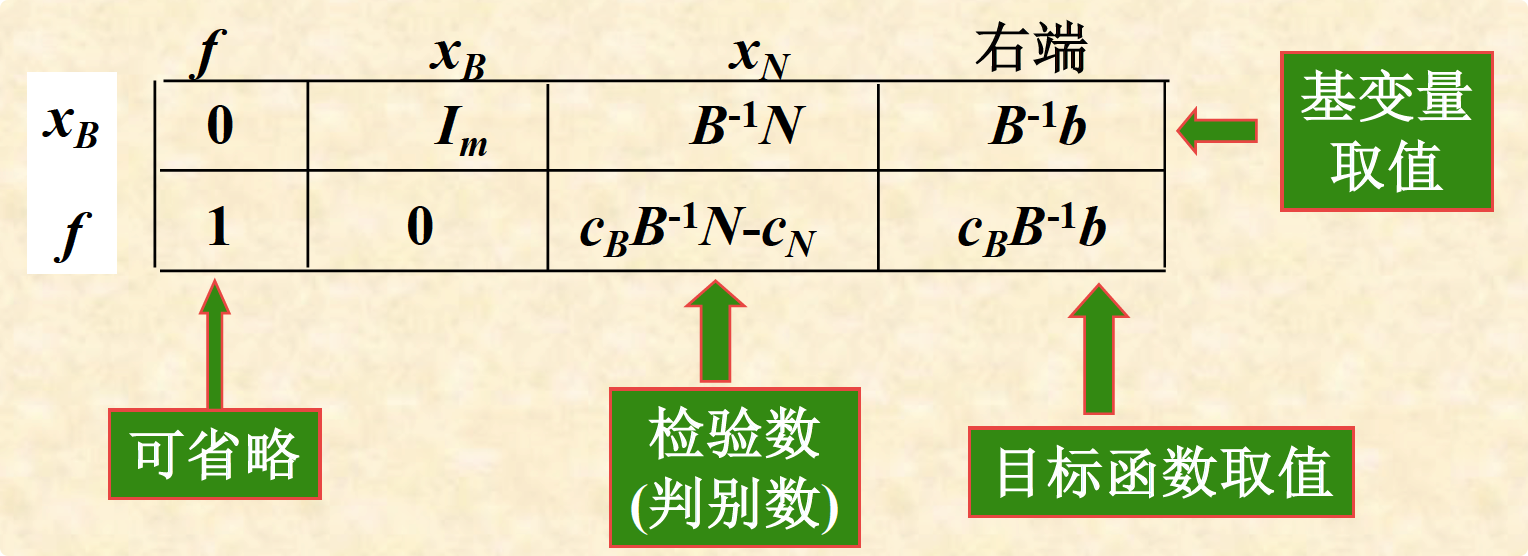
\includegraphics[width=0.8\textwidth]{./figures/img1.png}
        \caption{单纯形表 \label{fig1}}
    \end{figure}
\end{note}
